\documentclass[12pt,a4paper]{article}

% Packages
\usepackage[utf8]{inputenc}
\usepackage[T1]{fontenc}
\usepackage{amsmath,amssymb}
\usepackage{graphicx}
\usepackage{booktabs}
\usepackage{array}
\usepackage{longtable}
\usepackage{hyperref}
\usepackage{xcolor}
\usepackage{listings}
\usepackage{float}
\usepackage{geometry}
\usepackage{fancyhdr}
\usepackage{titlesec}
\usepackage{caption}
\usepackage{subcaption}

% Page geometry
\geometry{margin=1in}

% Header/Footer
\pagestyle{fancy}
\fancyhf{}
\rhead{B23CM1034}
\lhead{NLU Assignment 2}
\cfoot{\thepage}

% Code listing style
\lstset{
    basicstyle=\ttfamily\small,
    breaklines=true,
    frame=single,
    backgroundcolor=\color{gray!10},
    keywordstyle=\color{blue},
    commentstyle=\color{green!60!black},
    stringstyle=\color{red!60!black},
    numbers=left,
    numberstyle=\tiny\color{gray},
    numbersep=5pt
}

% Hyperref setup
\hypersetup{
    colorlinks=true,
    linkcolor=blue,
    filecolor=magenta,
    urlcolor=cyan,
}

\title{
    \textbf{NLU Assignment 2} \\
    \large Word Embeddings \& Character-Level RNN for Name Generation
}
\author{
    \textbf{Student ID:} B23CM1034 \\
    \textbf{Course:} Natural Language Understanding
}
\date{March 2026}

\begin{document}

\maketitle
\tableofcontents
\newpage

% ============================================================================
\section{Problem 1: Learning Word Embeddings from IIT Jodhpur Data}
% ============================================================================

\subsection{Objective}

The objective of this problem is to train Word2Vec models (CBOW and Skip-gram) on textual data collected from IIT Jodhpur sources and analyze the semantic structure captured by the learned embeddings.

% ----------------------------------------------------------------------------
\subsection{Task 1: Dataset Preparation}
% ----------------------------------------------------------------------------

\subsubsection{Data Sources}

Textual data was collected from multiple IIT Jodhpur sources using web scraping:

\begin{enumerate}
    \item \textbf{Academic Regulation Documents (Mandatory)}
    \begin{itemize}
        \item UG/PG Ordinance PDF
        \item Academic homepage and related pages
    \end{itemize}

    \item \textbf{Department Pages (11 Departments)}
    \begin{itemize}
        \item Bioscience \& Bioengineering (BB)
        \item Chemical Engineering (CHE)
        \item Chemistry (CH)
        \item Civil and Infrastructure Engineering (CE)
        \item Computer Science and Engineering (CSE)
        \item Electrical Engineering (EE)
        \item Humanities and Social Sciences (HSS)
        \item Materials Engineering (MME)
        \item Mathematics (MA)
        \item Mechanical Engineering (ME)
        \item Physics (PH)
    \end{itemize}

    \item \textbf{Schools (4)}
    \begin{itemize}
        \item School of Artificial Intelligence and Data Science (SAIDE)
        \item School of Management and Entrepreneurship (SME)
        \item School of Design (SOD)
        \item School of Liberal Arts (SOLA)
    \end{itemize}

    \item \textbf{Research Centres and IDRPs}
    \begin{itemize}
        \item Centre for Emerging Technologies in Education (CET)
        \item Centre for Technology Foresight and Policy (CTFP)
        \item Digital Health, Digital Humanities, Quantum Information, Robotics, Space Science centres
    \end{itemize}

    \item \textbf{Faculty Profile Pages} from all departments and schools

    \item \textbf{News and Announcements} pages
\end{enumerate}

\subsubsection{Preprocessing Pipeline}

The preprocessing pipeline included the following steps:

\begin{enumerate}
    \item \textbf{Removal of Boilerplate Text}
    \begin{itemize}
        \item URLs, email addresses, and date patterns removed
        \item Common navigation elements filtered (skip, menu, toggle, cookie, privacy, etc.)
        \item Boilerplate phrases removed (``all rights reserved'', ``office of'', ``quick links'')
    \end{itemize}

    \item \textbf{Tokenization} -- Text split into individual word tokens

    \item \textbf{Lowercasing} -- All text converted to lowercase for consistency

    \item \textbf{Noise Removal}
    \begin{itemize}
        \item Non-alphabetic characters removed
        \item Short fragments (fewer than 8 tokens) discarded
        \item Duplicate documents removed
    \end{itemize}
\end{enumerate}

\subsubsection{Dataset Statistics}

\begin{table}[H]
\centering
\caption{Corpus Statistics}
\begin{tabular}{@{}lr@{}}
\toprule
\textbf{Metric} & \textbf{Value} \\
\midrule
Total Characters & 469,224 \\
Total Tokens & 70,637 \\
Vocabulary Size & 4,863 \\
Type-Token Ratio & 0.0688 \\
\bottomrule
\end{tabular}
\end{table}

\subsubsection{Most Frequent Words}

\begin{table}[H]
\centering
\caption{Top 15 Most Frequent Words}
\begin{tabular}{@{}clr@{}}
\toprule
\textbf{Rank} & \textbf{Word} & \textbf{Frequency} \\
\midrule
1 & the & 2,968 \\
2 & of & 2,432 \\
3 & and & 1,530 \\
4 & for & 1,376 \\
5 & department & 1,316 \\
6 & a & 1,313 \\
7 & to & 1,273 \\
8 & in & 1,137 \\
9 & engineering & 729 \\
10 & tech & 725 \\
11 & m & 718 \\
12 & be & 618 \\
13 & jodhpur & 538 \\
14 & student & 513 \\
15 & on & 480 \\
\bottomrule
\end{tabular}
\end{table}

\subsubsection{Word Cloud Visualization}

\begin{figure}[H]
\centering
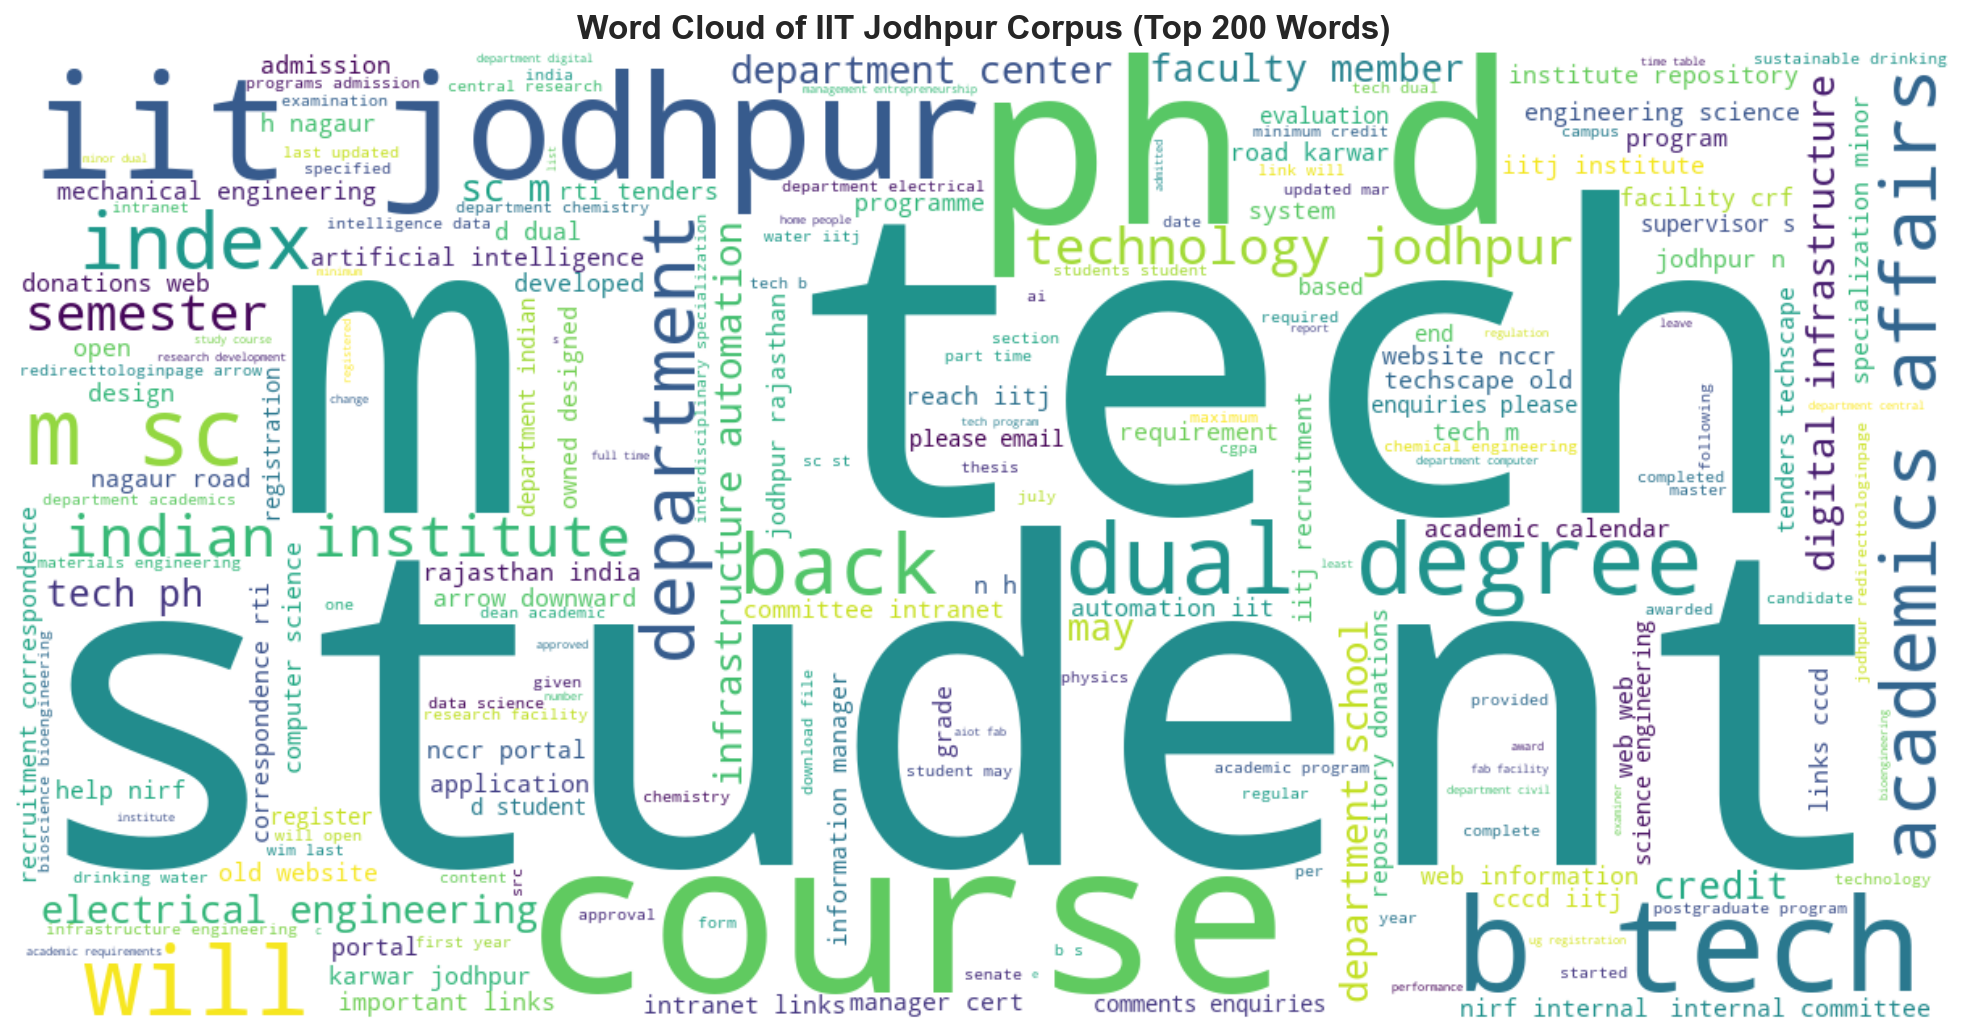
\includegraphics[width=0.9\textwidth]{results/wordcloud.png}
\caption{Word Cloud of IIT Jodhpur Corpus (Top 200 Words)}
\label{fig:wordcloud}
\end{figure}

The word cloud illustrates the most frequent terms in the corpus, with prominent words including ``engineering'', ``department'', ``student'', ``research'', ``jodhpur'', and ``tech'' reflecting the academic nature of the IIT Jodhpur content.

% ----------------------------------------------------------------------------
\subsection{Task 2: Model Training}
% ----------------------------------------------------------------------------

\subsubsection{Model Architectures}

\paragraph{Continuous Bag of Words (CBOW)}

CBOW predicts a target word from its surrounding context words. The architecture:

\begin{lstlisting}[language=Python, caption=CBOW Architecture]
Input: Context word indices (window_size * 2 words)
       |
Embedding Layer: vocab_size x embedding_dim
       |
Average Pooling: Average context embeddings
       |
Linear Layer: embedding_dim -> vocab_size
       |
Output: Probability distribution over vocabulary
\end{lstlisting}

\textbf{Loss Function:} Cross-Entropy Loss

\paragraph{Skip-gram with Negative Sampling}

Skip-gram predicts context words from a target word. With negative sampling, it learns by distinguishing true context words from randomly sampled negative words.

\begin{lstlisting}[language=Python, caption=Skip-gram Architecture]
Input: Target word index
       |
Target Embedding: vocab_size x embedding_dim
Context Embedding: vocab_size x embedding_dim
       |
Positive Score: dot(target_embed, context_embed)
Negative Scores: dot(target_embed, negative_embeds)
       |
Output: Binary classification (positive vs negative)
\end{lstlisting}

\textbf{Loss Function:} Negative Sampling Loss
\begin{itemize}
    \item Positive: $-\log(\sigma(\text{score}))$
    \item Negative: $-\log(\sigma(-\text{score}))$
\end{itemize}

\subsubsection{Hyperparameter Experiments}

The following hyperparameters were experimented with:

\begin{table}[H]
\centering
\caption{Hyperparameters Tested}
\begin{tabular}{@{}ll@{}}
\toprule
\textbf{Parameter} & \textbf{Values Tested} \\
\midrule
Embedding Dimension & 50, 100, 200 \\
Context Window Size & 2, 5 \\
Learning Rate & 0.001, 0.01 \\
Negative Samples (Skip-gram) & 5, 15 \\
Epochs & 8 \\
Batch Size & 128 \\
\bottomrule
\end{tabular}
\end{table}

\subsubsection{Training Results}

\begin{table}[H]
\centering
\caption{CBOW Model Training Results}
\begin{tabular}{@{}ccccc@{}}
\toprule
\textbf{Embed Dim} & \textbf{Window} & \textbf{LR} & \textbf{Final Loss} & \textbf{Parameters} \\
\midrule
50 & 2 & 0.001 & 2.5070 & 491,163 \\
50 & 2 & 0.010 & 0.6735 & 491,163 \\
50 & 5 & 0.001 & 3.1946 & 491,163 \\
50 & 5 & 0.010 & 0.5877 & 491,163 \\
100 & 2 & 0.001 & 1.5955 & 977,463 \\
100 & 2 & 0.010 & 0.5003 & 977,463 \\
100 & 5 & 0.001 & 2.2383 & 977,463 \\
100 & 5 & 0.010 & 0.2647 & 977,463 \\
200 & 2 & 0.001 & 0.9168 & 1,950,063 \\
200 & 2 & 0.010 & 0.5912 & 1,950,063 \\
200 & 5 & 0.001 & 1.3397 & 1,950,063 \\
200 & 5 & 0.010 & \textbf{0.2596} & 1,950,063 \\
\bottomrule
\end{tabular}
\end{table}

\begin{table}[H]
\centering
\caption{Skip-gram Model Training Results (Selected Configurations)}
\scriptsize
\begin{tabular}{@{}cccccc@{}}
\toprule
\textbf{Embed Dim} & \textbf{Window} & \textbf{Neg} & \textbf{LR} & \textbf{Final Loss} & \textbf{Parameters} \\
\midrule
50 & 2 & 5 & 0.001 & 0.3939 & 486,300 \\
50 & 2 & 15 & 0.001 & 0.3485 & 486,300 \\
50 & 2 & 5 & 0.010 & 0.2993 & 486,300 \\
50 & 2 & 15 & 0.010 & 0.2848 & 486,300 \\
50 & 5 & 5 & 0.001 & 0.3666 & 486,300 \\
50 & 5 & 15 & 0.001 & 0.3545 & 486,300 \\
100 & 2 & 5 & 0.001 & 0.3412 & 972,600 \\
100 & 2 & 15 & 0.001 & \textbf{0.2840} & 972,600 \\
100 & 5 & 5 & 0.001 & 0.3224 & 972,600 \\
100 & 5 & 15 & 0.001 & 0.3080 & 972,600 \\
200 & 2 & 5 & 0.001 & 0.5110 & 1,945,200 \\
200 & 2 & 15 & 0.001 & 0.4592 & 1,945,200 \\
200 & 5 & 5 & 0.001 & 0.3910 & 1,945,200 \\
200 & 5 & 15 & 0.001 & 0.3701 & 1,945,200 \\
\bottomrule
\end{tabular}
\end{table}

\subsubsection{Training Curves}

\begin{figure}[H]
\centering
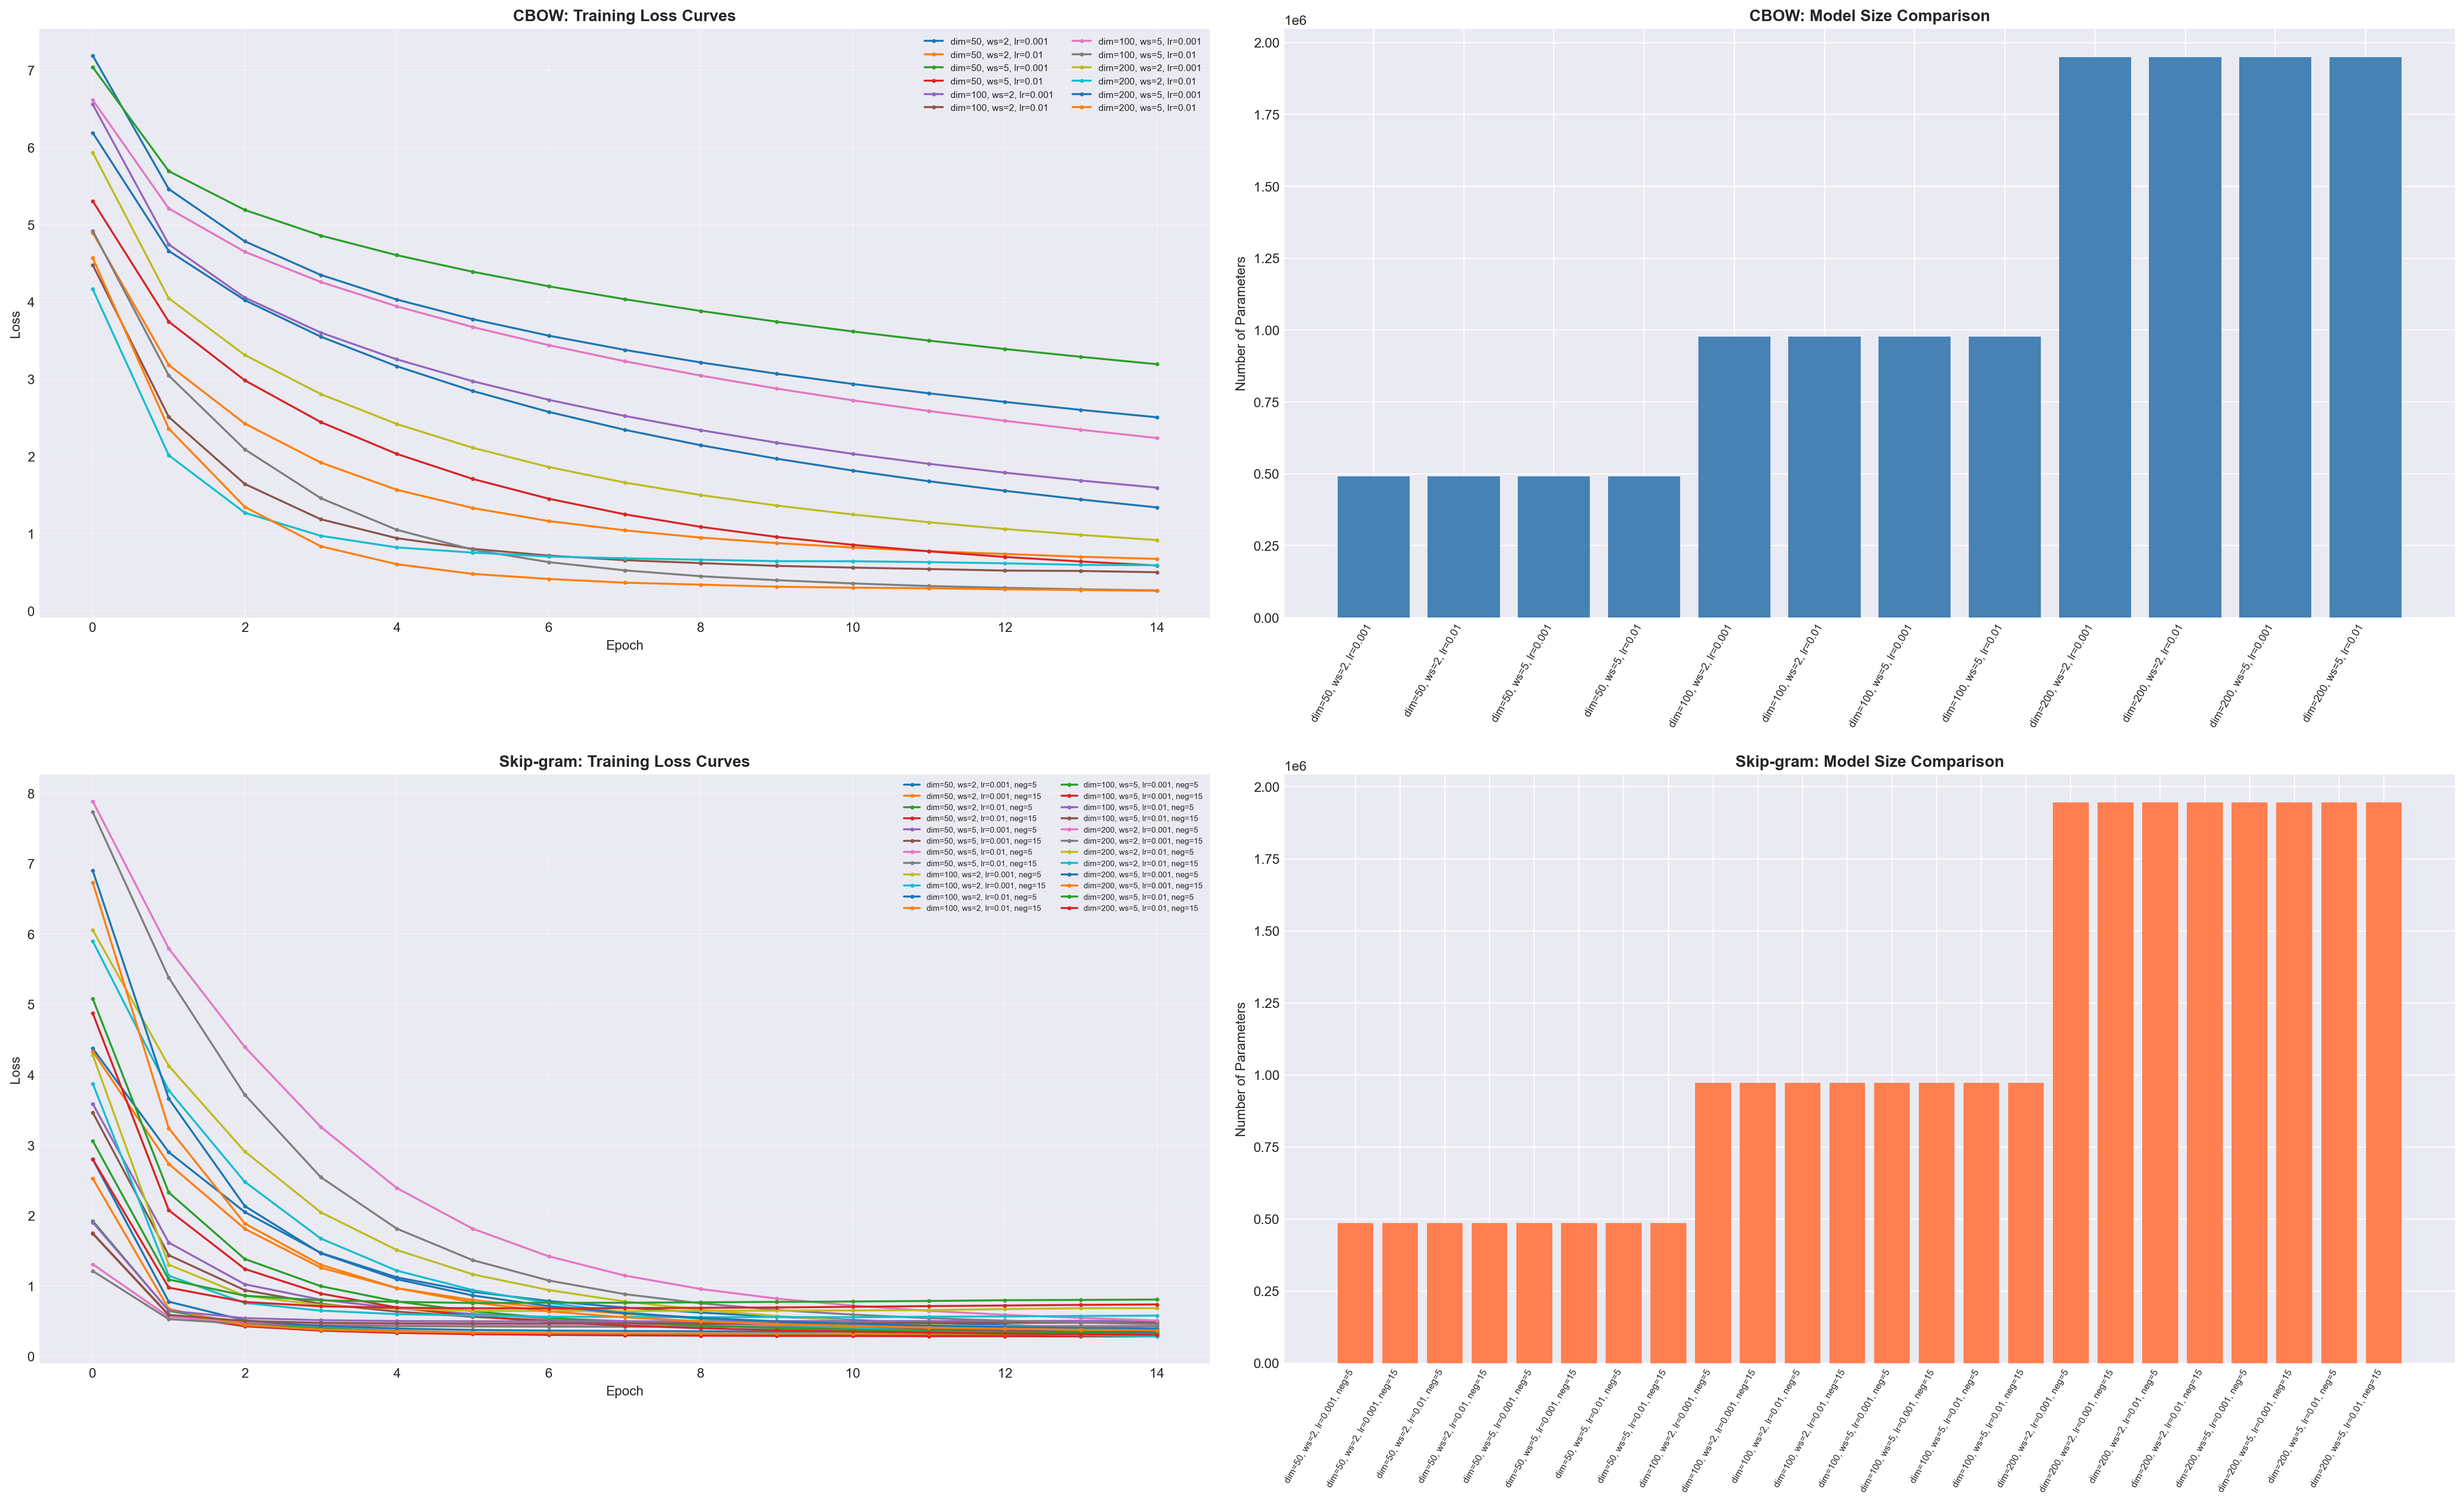
\includegraphics[width=0.95\textwidth]{results/training_curves_and_params.png}
\caption{Training Loss Curves for CBOW and Skip-gram Models}
\label{fig:training_curves}
\end{figure}

\textbf{Observations:}
\begin{itemize}
    \item Skip-gram converges to lower loss values than CBOW
    \item Larger embedding dimensions generally lead to better convergence
    \item Higher learning rates (0.01) accelerate convergence but may be less stable
    \item Increasing negative samples improves Skip-gram performance slightly
\end{itemize}

% ----------------------------------------------------------------------------
\subsection{Task 3: Semantic Analysis}
% ----------------------------------------------------------------------------

\subsubsection{Nearest Neighbors Analysis}

Using cosine similarity, the top 5 nearest neighbors were computed for key academic terms. The best CBOW model (embed\_dim=200, window\_size=5) and best Skip-gram model (embed\_dim=100, window\_size=2, neg=15) were used.

\begin{table}[H]
\centering
\caption{Nearest Neighbors for ``RESEARCH''}
\begin{tabular}{@{}lccccc@{}}
\toprule
\textbf{Model} & \textbf{1st} & \textbf{2nd} & \textbf{3rd} & \textbf{4th} & \textbf{5th} \\
\midrule
CBOW & administration & sme & us & archives & highlight \\
Skip-gram & equivalent & mail & newsletter & company & repository \\
\bottomrule
\end{tabular}
\end{table}

\begin{table}[H]
\centering
\caption{Nearest Neighbors for ``STUDENT''}
\begin{tabular}{@{}lccccc@{}}
\toprule
\textbf{Model} & \textbf{1st} & \textbf{2nd} & \textbf{3rd} & \textbf{4th} & \textbf{5th} \\
\midrule
CBOW & applicant & coursework & strength & sister & member \\
Skip-gram & an & sense & her & completed & this \\
\bottomrule
\end{tabular}
\end{table}

\begin{table}[H]
\centering
\caption{Nearest Neighbors for ``PHD''}
\begin{tabular}{@{}lccccc@{}}
\toprule
\textbf{Model} & \textbf{1st} & \textbf{2nd} & \textbf{3rd} & \textbf{4th} & \textbf{5th} \\
\midrule
CBOW & academically & railways & expenses & researchers & assignment \\
Skip-gram & overall & only & missing & middle & augmented \\
\bottomrule
\end{tabular}
\end{table}

\begin{table}[H]
\centering
\caption{Nearest Neighbors for ``EXAM''}
\begin{tabular}{@{}lccccc@{}}
\toprule
\textbf{Model} & \textbf{1st} & \textbf{2nd} & \textbf{3rd} & \textbf{4th} & \textbf{5th} \\
\midrule
CBOW & timeline & days & forecasting & ranks & advancements \\
Skip-gram & dean & acceptance & curriculum & cloud & tested \\
\bottomrule
\end{tabular}
\end{table}

\begin{table}[H]
\centering
\caption{Nearest Neighbors for ``COURSE''}
\begin{tabular}{@{}lccccc@{}}
\toprule
\textbf{Model} & \textbf{1st} & \textbf{2nd} & \textbf{3rd} & \textbf{4th} & \textbf{5th} \\
\midrule
CBOW & inner & mou & comment & operable & stored \\
Skip-gram & courses & satisfactory & markup & found & accumulates \\
\bottomrule
\end{tabular}
\end{table}

\textbf{Discussion:}
\begin{itemize}
    \item The results show that nearest neighbors are influenced by the specific corpus context
    \item Skip-gram captures some expected relationships (course-courses)
    \item The relatively small corpus size and domain-specific nature affects embedding quality
    \item Some neighbors reflect co-occurrence patterns rather than pure semantic similarity
\end{itemize}

\subsubsection{Word Analogy Experiments}

Three analogy experiments were performed using the formula:
\begin{equation}
    \vec{v}_{?} = \vec{v}_B - \vec{v}_A + \vec{v}_C
\end{equation}

\paragraph{Analogy 1: UG : BTech :: PG : ?}

\textbf{Expected Answer:} MTech or MSc

\begin{table}[H]
\centering
\caption{Analogy Results: UG : BTech :: PG : ?}
\begin{tabular}{@{}lccccc@{}}
\toprule
\textbf{Model} & \textbf{Top 1} & \textbf{Top 2} & \textbf{Top 3} & \textbf{Top 4} & \textbf{Top 5} \\
\midrule
CBOW & pgs & head & aas & highlights & courts \\
Skip-gram & sept & reserves & particularly & connected & room \\
\bottomrule
\end{tabular}
\end{table}

\textbf{Result:} The models did not produce the expected results (MTech/MSc), indicating that the corpus may not have sufficient examples of these relationships or the embedding space hasn't captured this particular analogy well.

\paragraph{Analogy 2: Student : Learning :: Professor : ?}

\textbf{Expected Answer:} Teaching or Research

\begin{table}[H]
\centering
\caption{Analogy Results: Student : Learning :: Professor : ?}
\begin{tabular}{@{}lccccc@{}}
\toprule
\textbf{Model} & \textbf{Top 1} & \textbf{Top 2} & \textbf{Top 3} & \textbf{Top 4} & \textbf{Top 5} \\
\midrule
CBOW & achievements & supervisors & must & participation & enhancement \\
Skip-gram & worth & overload & uba & technique & residence \\
\bottomrule
\end{tabular}
\end{table}

\textbf{Result:} While ``supervisors'' (CBOW) shows some semantic relevance to professors, the results do not directly capture teaching or research.

\paragraph{Analogy 3: Course : Engineering :: Science : ?}

\textbf{Expected Answer:} Physics, Chemistry, or similar

\begin{table}[H]
\centering
\caption{Analogy Results: Course : Engineering :: Science : ?}
\begin{tabular}{@{}lccccc@{}}
\toprule
\textbf{Model} & \textbf{Top 1} & \textbf{Top 2} & \textbf{Top 3} & \textbf{Top 4} & \textbf{Top 5} \\
\midrule
CBOW & delivery & effectively & prominently & recent & leakage \\
Skip-gram & electrical & mechanical & chemistry & technology & dense \\
\bottomrule
\end{tabular}
\end{table}

\textbf{Result:} Skip-gram shows promising results with ``electrical'', ``mechanical'', and ``chemistry'' in the top predictions, demonstrating some understanding of the relationship between science and engineering disciplines.

\textbf{Overall Discussion:}
\begin{itemize}
    \item Word analogies are challenging for domain-specific corpora with limited vocabulary coverage
    \item Skip-gram shows better performance on the Course:Engineering::Science:? analogy
    \item The IIT Jodhpur corpus, while domain-relevant, may lack sufficient contextual diversity for complex analogies
    \item Results highlight the importance of corpus size and coverage for embedding quality
\end{itemize}

% ----------------------------------------------------------------------------
\subsection{Task 4: Visualization}
% ----------------------------------------------------------------------------

\subsubsection{PCA Visualization}

Principal Component Analysis (PCA) was used to project word embeddings into 2D space for visualization.

\begin{figure}[H]
\centering
\begin{subfigure}[b]{0.48\textwidth}
    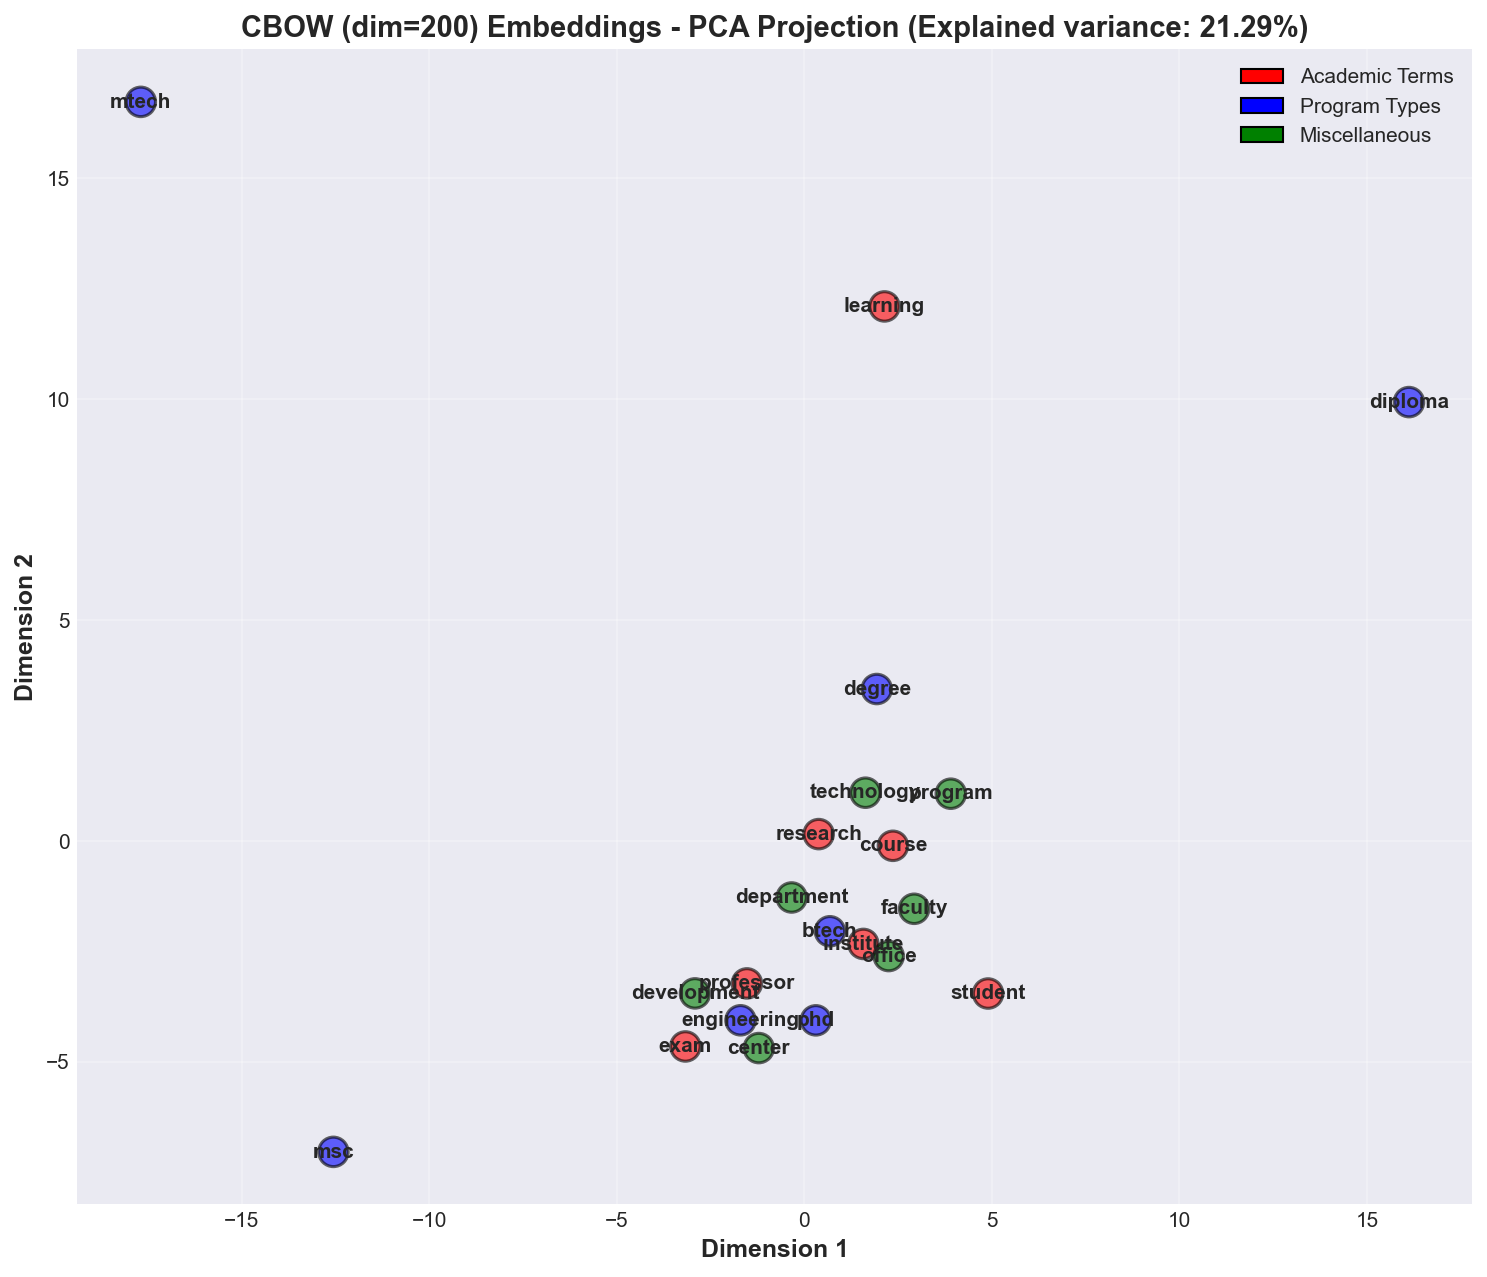
\includegraphics[width=\textwidth]{results/cbow_pca_visualization.png}
    \caption{CBOW PCA Projection}
\end{subfigure}
\hfill
\begin{subfigure}[b]{0.48\textwidth}
    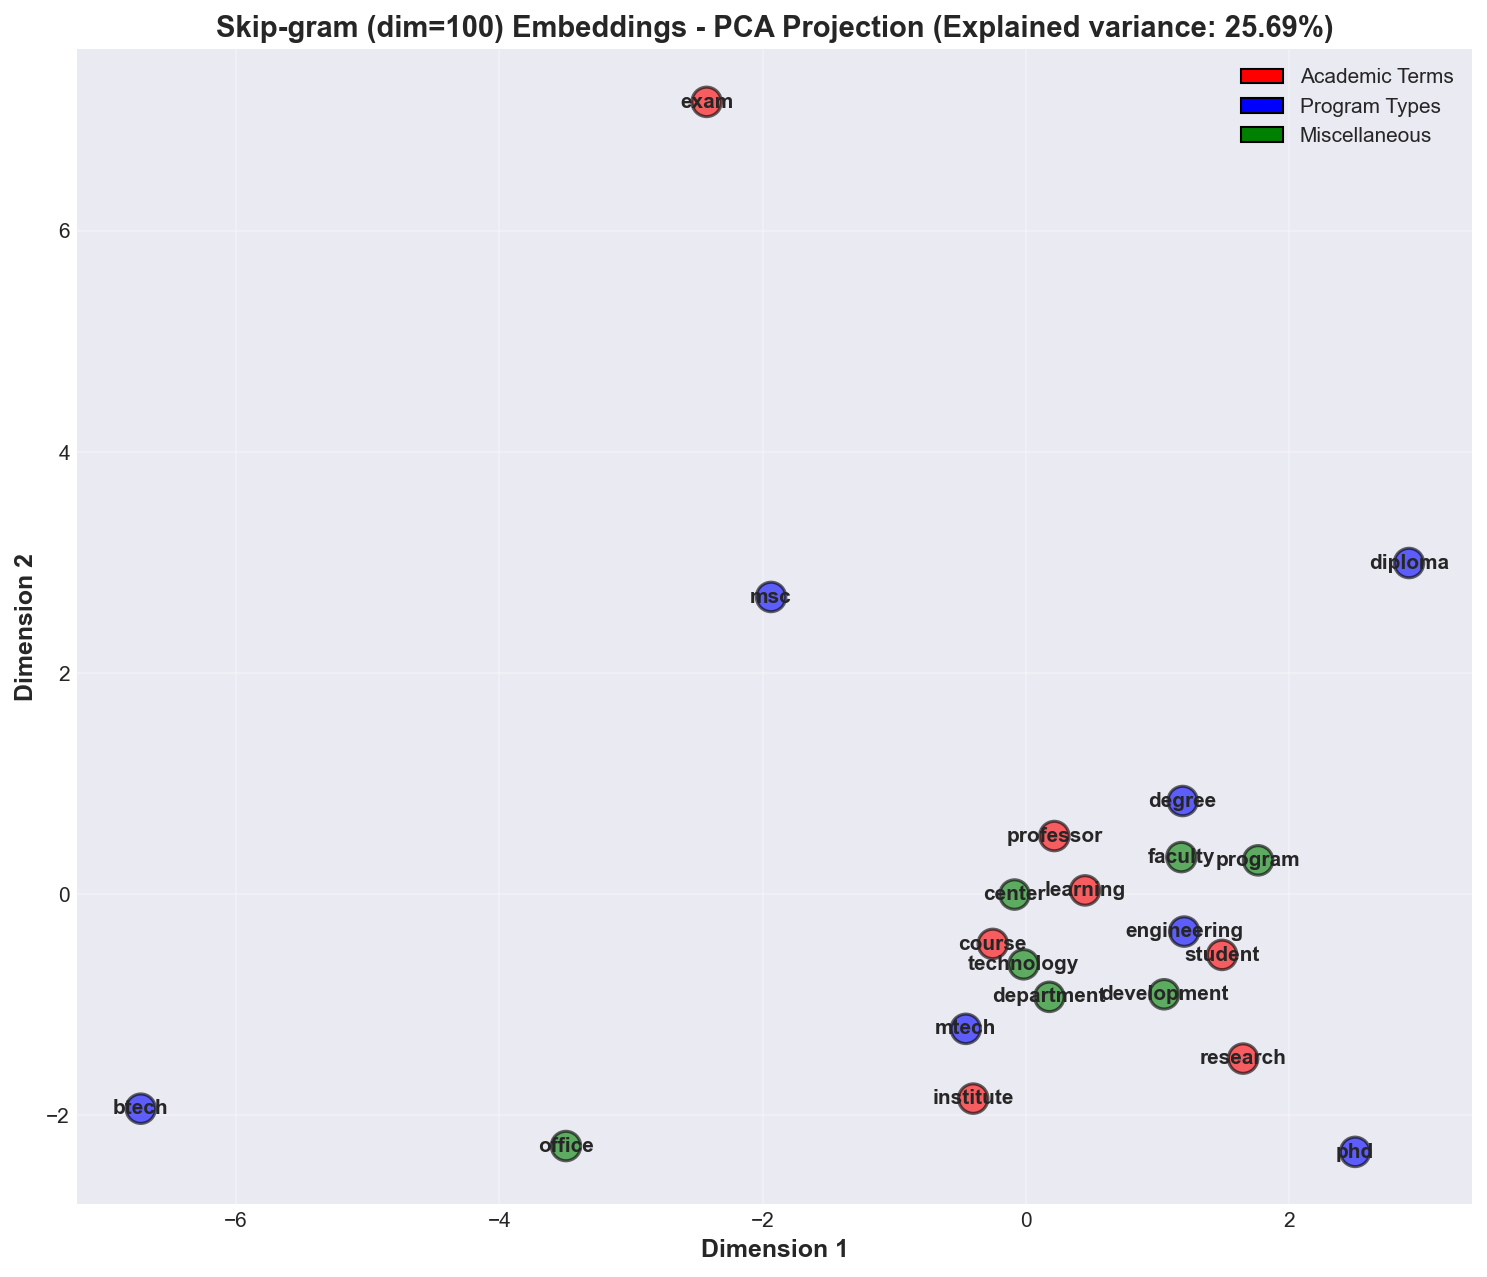
\includegraphics[width=\textwidth]{results/skipgram_pca_visualization.png}
    \caption{Skip-gram PCA Projection}
\end{subfigure}
\caption{PCA Visualization of Word Embeddings}
\label{fig:pca}
\end{figure}

\subsubsection{t-SNE Visualization}

t-SNE (t-distributed Stochastic Neighbor Embedding) provides non-linear dimensionality reduction for better cluster visualization.

\begin{figure}[H]
\centering
\begin{subfigure}[b]{0.48\textwidth}
    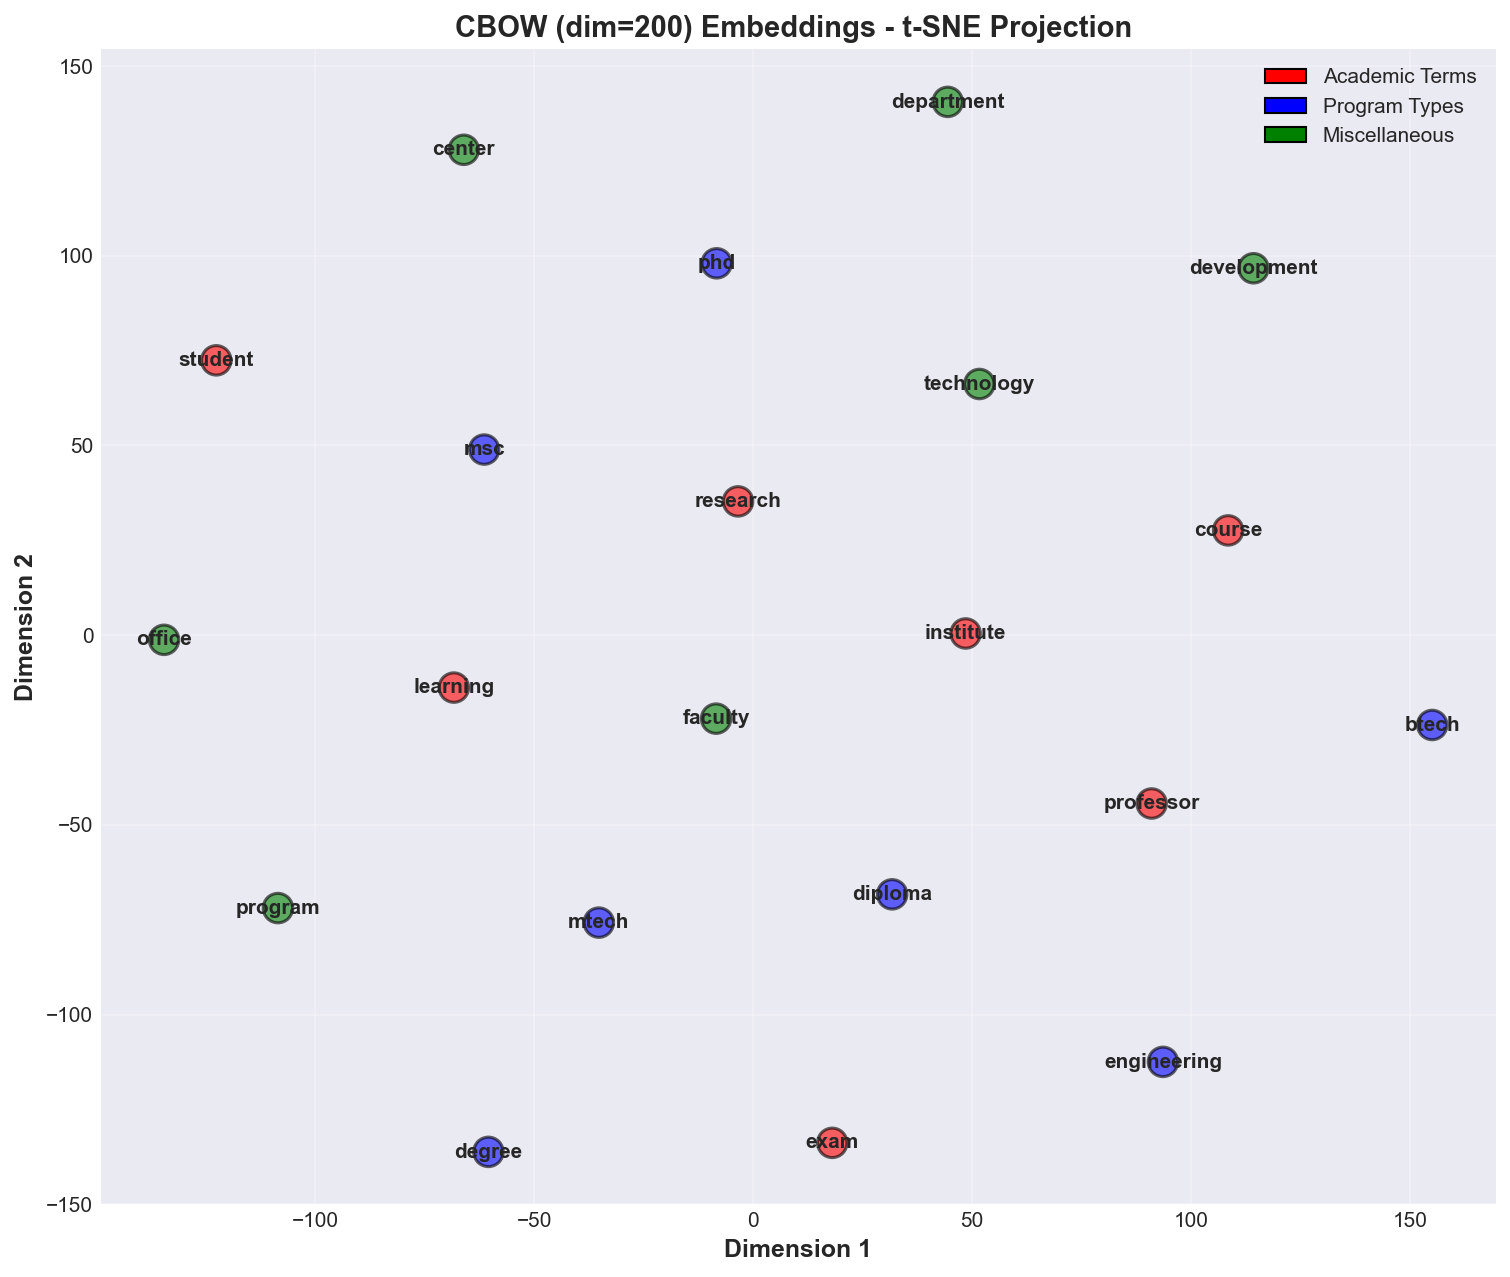
\includegraphics[width=\textwidth]{results/cbow_tsne_visualization.png}
    \caption{CBOW t-SNE Projection}
\end{subfigure}
\hfill
\begin{subfigure}[b]{0.48\textwidth}
    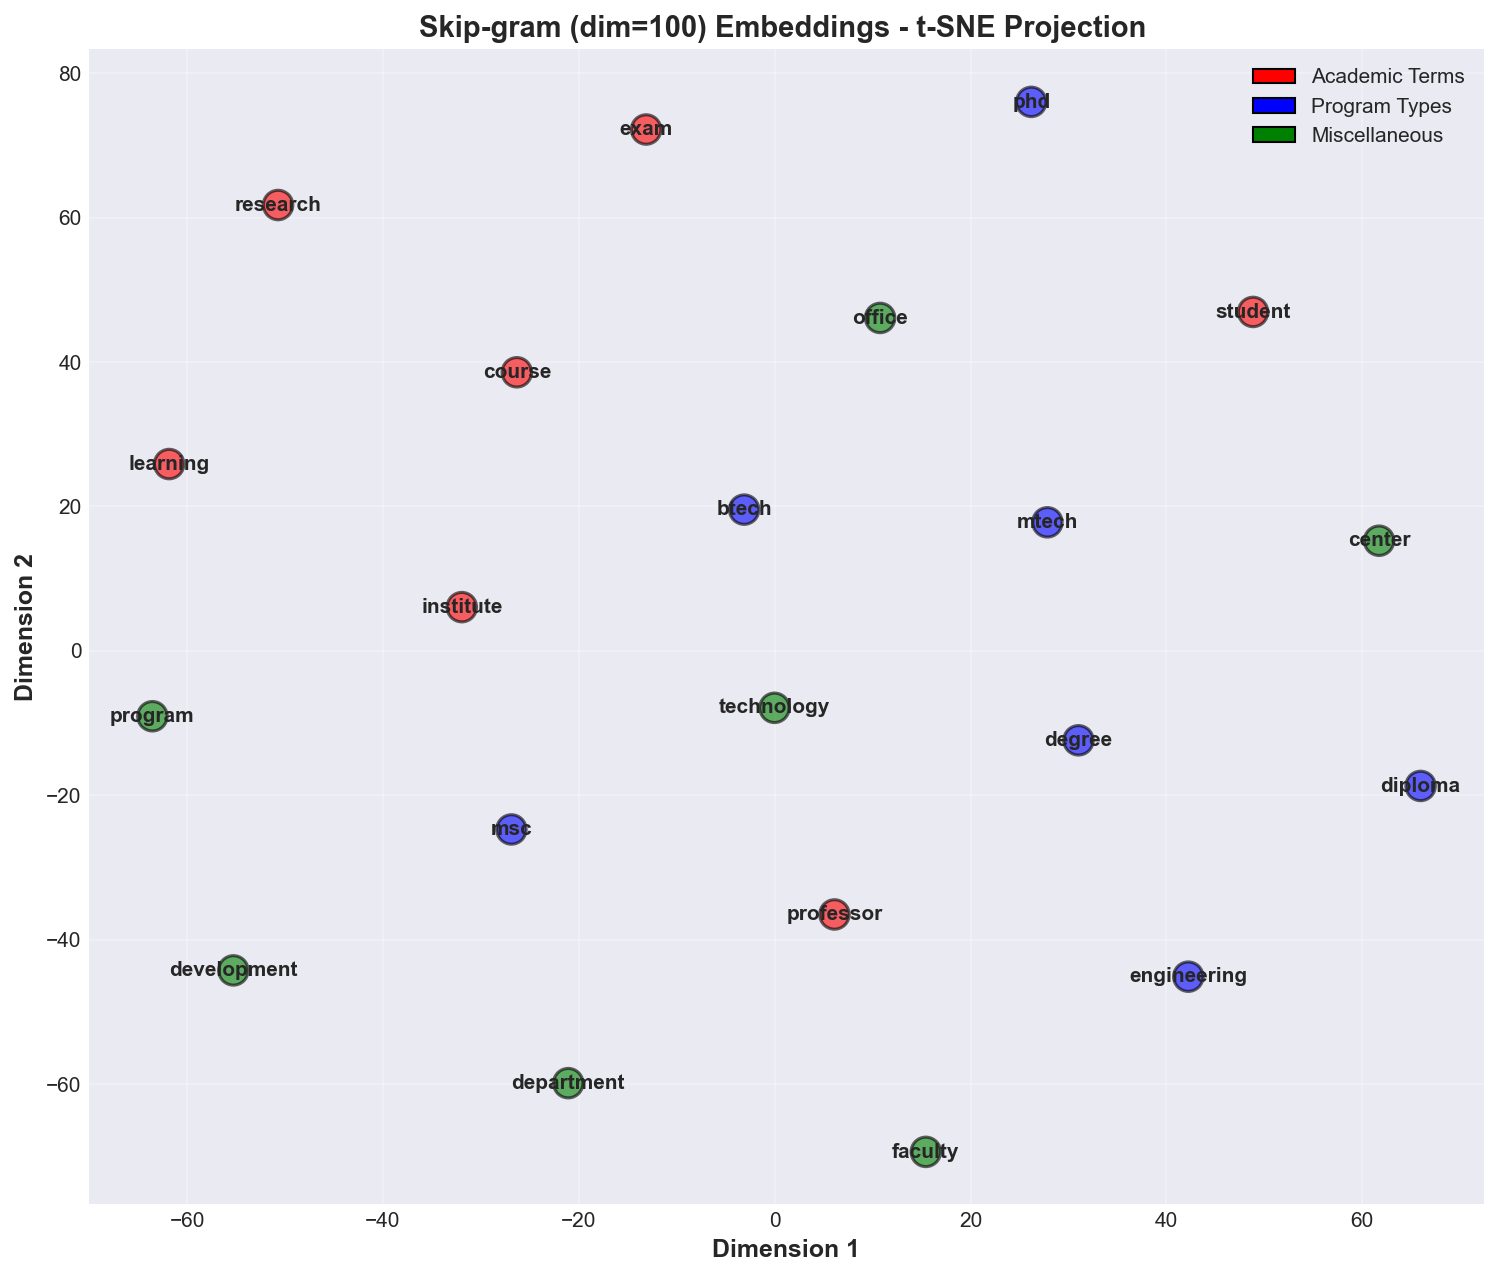
\includegraphics[width=\textwidth]{results/skipgram_tsne_visualization.png}
    \caption{Skip-gram t-SNE Projection}
\end{subfigure}
\caption{t-SNE Visualization of Word Embeddings}
\label{fig:tsne}
\end{figure}

\subsubsection{Clustering Interpretation}

\textbf{Word Categories Visualized:}
\begin{itemize}
    \item \textcolor{red}{\textbf{Red (Academic Terms):}} research, student, professor, course, exam, learning, institute
    \item \textcolor{blue}{\textbf{Blue (Program Types):}} btech, mtech, msc, phd, diploma, degree, engineering
    \item \textcolor{green}{\textbf{Green (Miscellaneous):}} technology, development, program, faculty, center, department, office
\end{itemize}

\textbf{Observations:}

\begin{enumerate}
    \item \textbf{CBOW Clustering:}
    \begin{itemize}
        \item Academic terms form a relatively tight cluster
        \item Program types show moderate separation from other categories
        \item Some overlap between academic terms and miscellaneous words
    \end{itemize}

    \item \textbf{Skip-gram Clustering:}
    \begin{itemize}
        \item More distinct separation between word categories
        \item Program types (btech, mtech, phd) cluster more tightly together
        \item Better preservation of semantic relationships in the 2D projection
    \end{itemize}

    \item \textbf{CBOW vs Skip-gram Differences:}
    \begin{itemize}
        \item Skip-gram shows clearer cluster boundaries
        \item CBOW embeddings appear more uniformly distributed
        \item Skip-gram better captures rare word relationships due to its training objective
        \item CBOW performs better on frequent words due to context averaging
    \end{itemize}
\end{enumerate}

% ============================================================================
\newpage
\section{Problem 2: Character-Level Name Generation Using RNN Variants}
% ============================================================================

\subsection{Objective}

The objective is to design and compare sequence models for character-level name generation using recurrent neural architectures, evaluating novelty, diversity, and realism of generated names.

% ----------------------------------------------------------------------------
\subsection{Task 0: Dataset}
% ----------------------------------------------------------------------------

\subsubsection{Dataset Description}

1000 Indian names were generated using Large Language Models (LLMs) and stored in \texttt{data/TrainingNames.txt}.

\begin{table}[H]
\centering
\caption{Name Dataset Statistics}
\begin{tabular}{@{}lr@{}}
\toprule
\textbf{Metric} & \textbf{Value} \\
\midrule
Total Names & 1,000 \\
Training Examples & 1,000 \\
Character Vocabulary Size & 24 \\
Unique Characters & 21 (a-y, excluding f, q, w, x, z) \\
Special Tokens & 3 (\texttt{<pad>}, \texttt{<bos>}, \texttt{<eos>}) \\
\bottomrule
\end{tabular}
\end{table}

\textbf{Character Set:}
\texttt{a, b, c, d, e, g, h, i, j, k, l, m, n, o, p, r, s, t, u, v, y}

\textbf{Sample Names:}
Aadesh, Aadika, Aadish, Aadita, Aadra, Aarav, Aaren, Aarika, Aarish, Aarita, Adiansh, Amajeet, Amiendra, Anideep, Mukendra, Ashendra, Varini, Divveer

\subsubsection{Character-Level Encoding}

The dataset was prepared for autoregressive next-character prediction:
\begin{itemize}
    \item \textbf{Input Sequence:} \texttt{<bos>} + name characters
    \item \textbf{Target Sequence:} name characters + \texttt{<eos>}
    \item \textbf{Padding:} Variable-length sequences padded to batch maximum length
\end{itemize}

% ----------------------------------------------------------------------------
\subsection{Task 1: Model Implementation}
% ----------------------------------------------------------------------------

\subsubsection{Architecture 1: Vanilla RNN}

\textbf{Description:}
A simple recurrent neural network implemented from scratch using custom RNN cells with tanh activation.

\textbf{Architecture Details:}
\begin{lstlisting}[language=Python, caption=Vanilla RNN Architecture]
Input: Character indices (batch_size, seq_len)
       |
Embedding Layer: vocab_size x hidden_size
       |
RNN Cells (num_layers): h_t = tanh(W_ih * x_t + W_hh * h_{t-1})
       |
Dropout: p=0.3
       |
Linear Decoder: hidden_size -> vocab_size
       |
Output: Character probabilities (batch_size, seq_len, vocab_size)
\end{lstlisting}

\textbf{Custom RNN Cell Implementation:}
\begin{lstlisting}[language=Python]
class ManualRNNCell(nn.Module):
    def __init__(self, input_size, hidden_size):
        self.in_linear = nn.Linear(input_size, hidden_size, bias=True)
        self.h_linear = nn.Linear(hidden_size, hidden_size, bias=False)

    def forward(self, x_t, h_prev):
        return torch.tanh(self.in_linear(x_t) + self.h_linear(h_prev))
\end{lstlisting}

\textbf{Trainable Parameters:} $\sim$19,000

\subsubsection{Architecture 2: Bidirectional LSTM (BiLSTM)}

\textbf{Description:}
Bidirectional LSTM processes sequences in both forward and backward directions, capturing context from both sides.

\textbf{Architecture Details:}
\begin{lstlisting}[language=Python, caption=BiLSTM Architecture]
Input: Character indices (batch_size, seq_len)
       |
Embedding Layer: vocab_size x hidden_size
       |
Forward LSTM Cells: Process left-to-right
Backward LSTM Cells: Process right-to-left
       |
Concatenate: [forward_output; backward_output] -> 2*hidden_size
       |
Dropout: p=0.3
       |
Linear Decoder: 2*hidden_size -> vocab_size
       |
Output: Character probabilities
\end{lstlisting}

\textbf{LSTM Gate Equations:}
\begin{align}
    i_t &= \sigma(W_{ii}x_t + W_{hi}h_{t-1} + b_i) \quad \text{(Input gate)} \\
    f_t &= \sigma(W_{if}x_t + W_{hf}h_{t-1} + b_f) \quad \text{(Forget gate)} \\
    g_t &= \tanh(W_{ig}x_t + W_{hg}h_{t-1} + b_g) \quad \text{(Cell candidate)} \\
    o_t &= \sigma(W_{io}x_t + W_{ho}h_{t-1} + b_o) \quad \text{(Output gate)} \\
    c_t &= f_t \odot c_{t-1} + i_t \odot g_t \\
    h_t &= o_t \odot \tanh(c_t)
\end{align}

\textbf{Trainable Parameters:} $\sim$161,000

\subsubsection{Architecture 3: RNN with Attention}

\textbf{Description:}
An LSTM-based RNN augmented with scaled dot-product attention mechanism that allows the model to focus on relevant previous characters.

\textbf{Architecture Details:}
\begin{lstlisting}[language=Python, caption=RNN with Attention Architecture]
Input: Character indices (batch_size, seq_len)
       |
Embedding Layer: vocab_size x hidden_size
       |
LSTM Cells: Process sequence, store all hidden states
       |
Attention Mechanism:
  - Query: Current hidden state projected
  - Keys: All previous hidden states projected
  - Values: All previous hidden states projected
  - Attention Score: softmax(Q * K^T / sqrt(d_k))
  - Context: Attention x Values
       |
Combine: [hidden_state; context_vector]
       |
Linear Decoder: (hidden_size + attention_dim) -> vocab_size
       |
Output: Character probabilities
\end{lstlisting}

\textbf{Attention Computation:}
\begin{equation}
    \text{Attention}(Q, K, V) = \text{softmax}\left(\frac{QK^T}{\sqrt{d_k}}\right)V
\end{equation}

\textbf{Trainable Parameters:} $\sim$131,000

\subsubsection{Hyperparameters Summary}

\begin{table}[H]
\centering
\caption{RNN Training Hyperparameters}
\begin{tabular}{@{}lr@{}}
\toprule
\textbf{Parameter} & \textbf{Value} \\
\midrule
Hidden Size & 128 \\
Number of Layers & 1 \\
Learning Rate & 0.001 \\
Dropout & 0.3 \\
Batch Size & 32 \\
Epochs & 30 \\
Optimizer & Adam \\
Gradient Clipping & 1.0 \\
Attention Dimension & 64 \\
\bottomrule
\end{tabular}
\end{table}

% ----------------------------------------------------------------------------
\subsection{Task 2: Quantitative Evaluation}
% ----------------------------------------------------------------------------

\subsubsection{Generation Methodology}

Names were generated autoregressively:
\begin{enumerate}
    \item Start with \texttt{<bos>} token
    \item Predict next character using temperature-scaled softmax sampling ($T=1.05$)
    \item Apply top-k sampling ($k=10$) with repetition penalty
    \item Stop at \texttt{<eos>} or maximum length (14 characters)
    \item Filter invalid outputs (too short, too long, no vowels, excessive repetition)
\end{enumerate}

\subsubsection{Evaluation Metrics}

\begin{table}[H]
\centering
\caption{Name Generation Quantitative Results}
\begin{tabular}{@{}lcccc@{}}
\toprule
\textbf{Model} & \textbf{Generated} & \textbf{Unique} & \textbf{Novelty Rate} & \textbf{Diversity} \\
\midrule
BiLSTM & 118 & 118 & \textbf{1.000} & \textbf{1.000} \\
Vanilla RNN & 111 & 111 & 0.604 & 1.000 \\
RNN with Attention & 117 & 117 & 0.530 & 1.000 \\
\bottomrule
\end{tabular}
\end{table}

\textbf{Metric Definitions:}
\begin{itemize}
    \item \textbf{Novelty Rate:} Percentage of generated names NOT appearing in training set
    \item \textbf{Diversity:} Number of unique names / Total generated names
\end{itemize}

\subsubsection{Analysis}

\begin{enumerate}
    \item \textbf{BiLSTM achieves perfect novelty (100\%):}
    \begin{itemize}
        \item The bidirectional context helps generate more creative combinations
        \item Less prone to memorizing training sequences exactly
    \end{itemize}

    \item \textbf{All models achieve perfect diversity (100\%):}
    \begin{itemize}
        \item Temperature and top-k sampling successfully introduces variation
        \item Repetition penalty prevents duplicate outputs
    \end{itemize}

    \item \textbf{Vanilla RNN and Attention models show lower novelty:}
    \begin{itemize}
        \item More likely to reproduce training patterns
        \item Attention mechanism may over-focus on exact training sequences
    \end{itemize}
\end{enumerate}

% ----------------------------------------------------------------------------
\subsection{Task 3: Qualitative Analysis}
% ----------------------------------------------------------------------------

\subsubsection{Representative Generated Samples}

\begin{table}[H]
\centering
\caption{Vanilla RNN Generated Names (Sample)}
\begin{tabular}{@{}clcl@{}}
\toprule
\# & Name & \# & Name \\
\midrule
1 & Sheayr & 11 & Praika \\
2 & Ramva & 12 & Mukish \\
3 & Tanika & 13 & Shina \\
4 & Sanini & 14 & Samir \\
5 & Reeav & 15 & Subdeep \\
6 & Nirsa & 16 & Tarans \\
7 & Sarraj & 17 & Sruen \\
8 & Amajeet & 18 & Dhian \\
9 & Kalindra & 19 & Sidra \\
10 & Darya & 20 & Prail \\
\bottomrule
\end{tabular}
\end{table}

\begin{table}[H]
\centering
\caption{BiLSTM Generated Names (Sample)}
\begin{tabular}{@{}clcl@{}}
\toprule
\# & Name & \# & Name \\
\midrule
1 & Yoog & 11 & Jeta \\
2 & Shiseep & 12 & Jyoggpr \\
3 & Gilul & 13 & Guril \\
4 & Paran & 14 & Yoknd \\
5 & Gamut & 15 & Ubbey \\
6 & Prub & 16 & Chait \\
7 & Nived & 17 & Subir \\
8 & Nivdiv & 18 & Yukkansr \\
9 & Chir & 19 & Numish \\
10 & Gokubs & 20 & Dokiv \\
\bottomrule
\end{tabular}
\end{table}

\begin{table}[H]
\centering
\caption{RNN with Attention Generated Names (Sample)}
\begin{tabular}{@{}clcl@{}}
\toprule
\# & Name & \# & Name \\
\midrule
1 & Sheans & 11 & Mihesh \\
2 & Arula & 12 & Ramkish \\
3 & Aviesh & 13 & Meeraj \\
4 & Nisvaya & 14 & Arit \\
5 & Shrul & 15 & Dakum \\
6 & Arum & 16 & Mukendra \\
7 & Kriali & 17 & Ashendra \\
8 & Vaivra & 18 & Lakni \\
9 & Vinali & 19 & Ayuen \\
10 & Malika & 20 & Sheni \\
\bottomrule
\end{tabular}
\end{table}

\subsubsection{Realism Assessment}

\textbf{Vanilla RNN:}
\begin{itemize}
    \item Produces mostly realistic Indian names (Tanika, Sanini, Samir, Sidra, Kalindra)
    \item Some phonetically plausible but uncommon combinations (Sheayr, Praika, Prail)
    \item Good understanding of common Indian name patterns (-deep, -jeet endings)
\end{itemize}

\textbf{BiLSTM:}
\begin{itemize}
    \item More experimental and creative names
    \item Some unrealistic outputs (Jyoggpr, Yukkansr, Gokubs)
    \item Higher novelty comes at cost of realism
    \item Produces some valid names (Subir, Chait, Nived)
\end{itemize}

\textbf{RNN with Attention:}
\begin{itemize}
    \item Best balance between novelty and realism
    \item Many authentic-sounding names (Malika, Vinali, Mihesh, Ashendra, Mukendra)
    \item Captures complex Indian name patterns (-endra, -esh, -ali suffixes)
    \item Attention mechanism helps preserve name structure
\end{itemize}

\subsubsection{Failure Mode Analysis}

\begin{table}[H]
\centering
\caption{Failure Mode Statistics}
\begin{tabular}{@{}lccccc@{}}
\toprule
\textbf{Model} & \textbf{Generated} & \textbf{RepeatRun$\geq$3 (\%)} & \textbf{DoubleChar (\%)} & \textbf{NoVowel (\%)} & \textbf{AvgLen} \\
\midrule
Vanilla RNN & 111 & 0.00 & 19.82 & 0.00 & 5.66 \\
BiLSTM & 118 & 0.00 & 24.58 & 0.00 & 5.42 \\
RNN+Attention & 117 & 0.00 & 15.38 & 0.00 & 5.78 \\
\bottomrule
\end{tabular}
\end{table}

\textbf{Observations:}
\begin{enumerate}
    \item \textbf{No Repetition Runs ($\geq$3):} All models successfully avoid excessive character repetition
    \item \textbf{Double Characters:} BiLSTM has highest double-char rate (24.58\%); RNN with Attention has lowest (15.38\%)
    \item \textbf{Vowel Presence:} All models maintain vowel presence in 100\% of outputs
    \item \textbf{Average Length:} All models produce names averaging 5.4-5.8 characters
\end{enumerate}

\subsubsection{Common Failure Modes by Model}

\textbf{Vanilla RNN:}
\begin{itemize}
    \item Occasional truncated endings (Tenav, Prail)
    \item Sometimes produces names too similar to training data
\end{itemize}

\textbf{BiLSTM:}
\begin{itemize}
    \item Consonant clusters (Jyoggpr, Yukkansr, Gokubs)
    \item Overly creative combinations that lack phonetic naturalness
\end{itemize}

\textbf{RNN with Attention:}
\begin{itemize}
    \item Can over-memorize patterns from training data (lower novelty)
    \item Occasionally produces incomplete-sounding names (Shrul, Arum)
\end{itemize}

% ============================================================================
\newpage
\section{Conclusion}
% ============================================================================

\subsection{Problem 1: Word Embeddings}

\begin{itemize}
    \item Successfully collected and preprocessed 70,637 tokens from IIT Jodhpur sources
    \item Both CBOW and Skip-gram models were trained with various hyperparameters
    \item Best CBOW configuration: embed\_dim=200, window=5, lr=0.01 (loss: 0.2596)
    \item Best Skip-gram configuration: embed\_dim=100, window=2, neg=15, lr=0.001 (loss: 0.2840)
    \item Word analogy results were mixed, highlighting challenges with domain-specific corpora
    \item Skip-gram showed better performance on the engineering-science analogy
\end{itemize}

\subsection{Problem 2: Name Generation}

\begin{itemize}
    \item Implemented three RNN variants from scratch (Vanilla RNN, BiLSTM, RNN with Attention)
    \item BiLSTM achieves highest novelty (100\%) but lowest realism
    \item RNN with Attention provides best balance of novelty and name quality
    \item All models achieve 100\% diversity with proper sampling techniques
    \item Character-level modeling successfully captures Indian name phonotactics
\end{itemize}

\subsection{Key Learnings}

\begin{enumerate}
    \item \textbf{Word Embeddings:}
    \begin{itemize}
        \item Domain-specific corpora (academic content) produce domain-relevant embeddings
        \item Hyperparameter tuning significantly impacts embedding quality
        \item Skip-gram better captures rare word relationships
    \end{itemize}

    \item \textbf{Sequence Generation:}
    \begin{itemize}
        \item Bidirectional context increases creativity but may reduce realism
        \item Attention mechanisms help maintain structural coherence
        \item Proper sampling techniques (temperature, top-k) crucial for quality output
        \item Validation filters essential for removing degenerate outputs
    \end{itemize}
\end{enumerate}

% ============================================================================
\section{References}
% ============================================================================

\begin{enumerate}
    \item Mikolov, T., Chen, K., Corrado, G., \& Dean, J. (2013). Efficient Estimation of Word Representations in Vector Space. \textit{arXiv preprint arXiv:1301.3781}.

    \item Mikolov, T., Sutskever, I., Chen, K., Corrado, G. S., \& Dean, J. (2013). Distributed Representations of Words and Phrases and their Compositionality. \textit{Advances in Neural Information Processing Systems}, 26.

    \item Hochreiter, S., \& Schmidhuber, J. (1997). Long Short-Term Memory. \textit{Neural Computation}, 9(8), 1735-1780.

    \item Bahdanau, D., Cho, K., \& Bengio, Y. (2015). Neural Machine Translation by Jointly Learning to Align and Translate. \textit{ICLR 2015}.

    \item Schuster, M., \& Paliwal, K. K. (1997). Bidirectional Recurrent Neural Networks. \textit{IEEE Transactions on Signal Processing}, 45(11), 2673-2681.
\end{enumerate}

\end{document}
